\documentclass[conference]{IEEEtran}
\IEEEoverridecommandlockouts
% The preceding line is only needed to identify funding in the first footnote. If that is unneeded, please comment it out.
%Template version as of 6/27/2024

\usepackage{cite}
\usepackage{amsmath,amssymb,amsfonts}
\usepackage{algorithmic}
\usepackage{float}
\usepackage{graphicx}
\usepackage[colorlinks=true, urlcolor=blue]{hyperref}
\usepackage{listings}
\usepackage{multirow}
\usepackage{textcomp}
\usepackage{xcolor}
\def\BibTeX{{\rm B\kern-.05em{\sc i\kern-.025em b}\kern-.08em
    T\kern-.1667em\lower.7ex\hbox{E}\kern-.125emX}}

\makeatletter
\def\subsubsection{\@startsection{subsubsection}{3}{\z@}%
  {1.5ex plus 1ex minus .2ex}%
  {1ex plus .2ex}%
  {\normalfont\normalsize}}
\makeatother
\pagestyle{plain}

\begin{document}

\title{
    CSE 620 Project 1: Gradient Descent Variants\\[0.5em]
    \Large Fall 2026\\[0.5em]
    \large \href{https://github.com/rlovett992/CSE_620_Fall26_Project1_Robert_John/tree/main}{Our Code}
}

\author{
    \IEEEauthorblockN{John Brittian}
    \and
    \IEEEauthorblockN{Robert Lovett}
}

\maketitle

\begin{abstract}
This report documents a wellthought-out and precise carrying out of the first project for CSE 620.
\end{abstract}

\begin{IEEEkeywords}
heuristics, gradient descent, optimization, fun
\end{IEEEkeywords}

\section{Introduction}
The objective of this project is to implement and explore several variants of the gradient descent optimization algorithm.
Each variant will be used to minimize each of the following functions. The only
constraint is that these functions are all of the form $f: \mathbb{R}^2 \to \mathbb{R}$,
so we're minimizing over the entire plane.

\begin{equation}
    f_1(x,y) = x^2 + y^2
\end{equation}

\begin{equation}
    f_2(x,y) = (1-x)^2 + 100(y - x^2)^2
\end{equation}

\begin{equation}
    f_3(x,y) = x^2 + y^2 + 10\cos{x} + 10\cos{y}
\end{equation}

We've implemented and experimented with:

\begin{enumerate}
    \item Vanilla Gradient Descent
    \item Newton's Method (w/ Hessian)
    \item AdaGrad
    \item Adam (w/ $\beta_1=0.9$, $\beta_2=0.999$, $\epsilon=1\mathrm{e}-8$)
\end{enumerate}

\section{Methods}

Here we describe in more detail the gradient descent algorithms used, and our
implementations of them.

\subsection{Gradient Descent Algorithms}

\subsubsection{Vanilla Gradient Descent}

This one isn't anything crazy. This algorithm simply starts with a random initial point
(here we use a fixed initial point for consistency), then iteratively updates
the point using the gradient of $f$:

\[
    \nabla f = \begin{bmatrix}
        \frac{\partial f}{\partial x} \\[0.5em]
        \frac{\partial f}{\partial y}
    \end{bmatrix}
\]

This algorithm in pseudocode looks like this:

\begin{algorithmic}[1]
    \STATE Initialize $(x,y) \gets (x_0,y_0)$
    \STATE Initialize $\alpha \gets \alpha_0$
    \FOR{$t=1,\ldots,T$}
        \STATE $(x,y) \gets (x,y) - \alpha \nabla f(x,y)$

    \ENDFOR
    \STATE \textbf{return} $(x,y)$
\end{algorithmic}

\subsubsection{Newton's Method (w/ Hessian)}

Newton's Method is a second-order optimization algorithm that uses both
the gradient and the Hessian matrix of $f$:

\[
    \boldmath{H}_f = \begin{bmatrix}
        \frac{\partial^2 f}{\partial x^2} & \frac{\partial^2 f}{\partial x \partial y} \\[0.5em]
        \frac{\partial^2 f}{\partial y \partial x} & \frac{\partial^2 f}{\partial y^2}
    \end{bmatrix}
\]

This algorithm in pseudocode looks like this:

\begin{algorithmic}[1]
    \STATE Initialize $(x,y) \gets (x_0,y_0)$
    \STATE Initialize $\alpha \gets \alpha_0$
    \FOR{$t=1,\ldots,T$}
        \STATE $(x,y) \gets (x,y) - \alpha H_f^{-1}(x,y) \nabla f(x,y)$

    \ENDFOR
    \STATE \textbf{return} $(x,y)$
\end{algorithmic}

\subsubsection{AdaGrad}

AdaGrad is an adaptive learning rate optimization algorithm that adjusts the learning rate for each parameter based on the historical gradients.
It accumulates the squared gradients and uses them to scale the learning rate.
Some implementations the entire outer product of past gradients with itself,
but ours uses only the diagonal of that matrix, which is much more
computationally efficient.

This algorithm in pseudocode looks like this:

\begin{algorithmic}[1]
    \STATE Initialize $(x,y) \gets (x_0,y_0)$
    \STATE Initialize $\alpha \gets \alpha_0$
    \STATE Initialize $g_{acc} \gets (0, 0)$
    \FOR{$t=1,\ldots,T$}
        \STATE $g \gets \nabla f(x,y)$
        \STATE $g_{acc} \gets g_{acc} + g \odot g$
        \STATE $(x,y) \gets (x,y) - \alpha \cdot \left(g_{acc}\right)^{\odot -\frac12} \cdot \nabla f(x,y)$
    \ENDFOR
    \STATE \textbf{return} $(x,y)$
\end{algorithmic}

where $\odot$ denotes the \href{https://en.wikipedia.org/wiki/Hadamard_product_(matrices)}{Hadamard operations}.

\subsubsection{Adam}

Adam is essentially an intelligent combination of AdaGrad with momentum. It tracks
an exponentially decaying average of past gradients and squared gradients, and uses these to adapt the learning rate for each parameter.
In this project we use the following values for Adam's unique hyperparameters:

\[\beta_1=0.9\qquad\beta_2=0.999\qquad\epsilon=1\mathrm{e}-8\]

This algorithm in pseudocode looks like this:

\begin{algorithmic}[1]
    \STATE Initialize $(x,y) \gets (x_0,y_0)$
    \STATE Initialize $\alpha \gets \alpha_0$
    \STATE Initialize $m \gets (0, 0)$
    \STATE Initialize $v \gets (0, 0)$
    \FOR{$t=1,\ldots,T$}
        \STATE $g \gets \nabla f(x,y)$
        \STATE $m \gets \beta_1 m + (1 - \beta_1)g$
        \STATE $v \gets \beta_2 v + (1 - \beta_2)\left(g \odot g\right)$
        \STATE $\hat{m} \gets \frac{m}{1 - \beta_1^t}$
        \STATE $\hat{v} \gets \frac{v}{1 - \beta_2^t}$
        \STATE $(x,y) \gets (x,y) - \alpha \cdot \left(\hat{m} \oslash \left(\sqrt{\hat{v}} + \epsilon\right)\right)$
    \ENDFOR
    \STATE \textbf{return} $(x,y)$
\end{algorithmic}

where $\oslash$ denotes the \href{https://en.wikipedia.org/wiki/Hadamard_product_(matrices)#Analogous_operations}{Hadamard division}.

\subsection{Our Code}

We wrote our scripts in Python and built the algorithms from (mostly) scratch.
They can be found in the appendix, findable from these links - \hyperref[lst:gradient_descent]{Gradient Descent},
\hyperref[lst:newtons_method]{Newton's Method}, \hyperref[lst:adagrad]{AdaGrad}, and \hyperref[lst:adam]{Adam}.

For running the code, first clone the \href{https://github.com/rlovett992/CSE_620_Fall26_Project1_Robert_John/tree/main}{repository}.
Next, simply running the script \texttt{run\_all.py} will generate all the results, plots, and data files.

\section{Results}
Running our code generated the following plots for each combination of algorithm and function.
Furthermore, we have complete, tabular results for each hyperparameter combination.

\subsection{Adagrad}

\subsubsection{Cosine Bumps}
\begin{figure}[H]
    \centering
    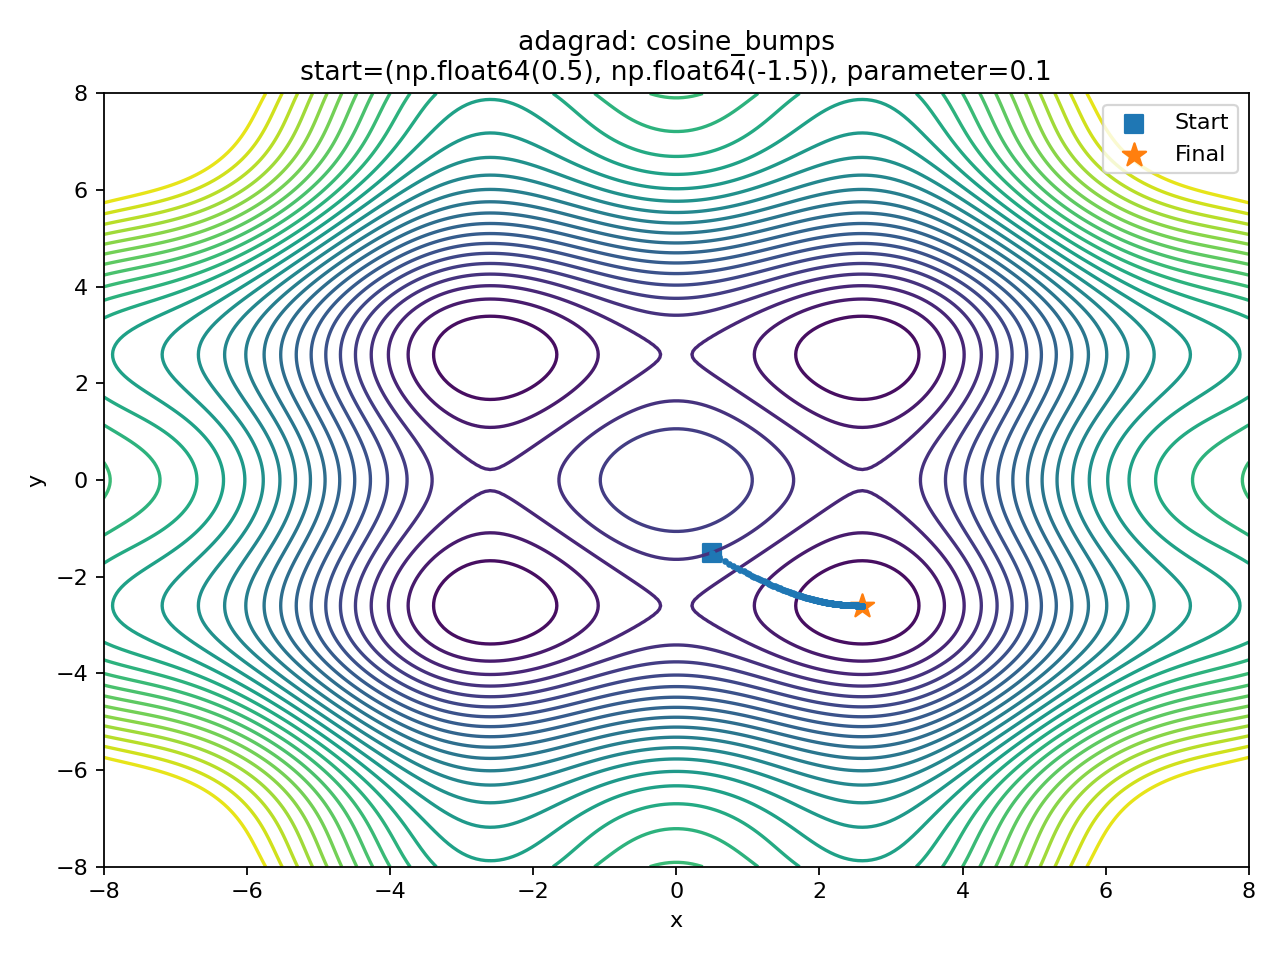
\includegraphics[width=0.40\textwidth]{output/adagrad/cosine_bumps_start_0.5_neg1.5_lr_0.1.png}
    \caption{Adagrad on the Cosine Bumps function}
    \label{fig:adagrad_cosine}
\end{figure}

\subsubsection{Quadratic}
\begin{figure}[H]
    \centering
    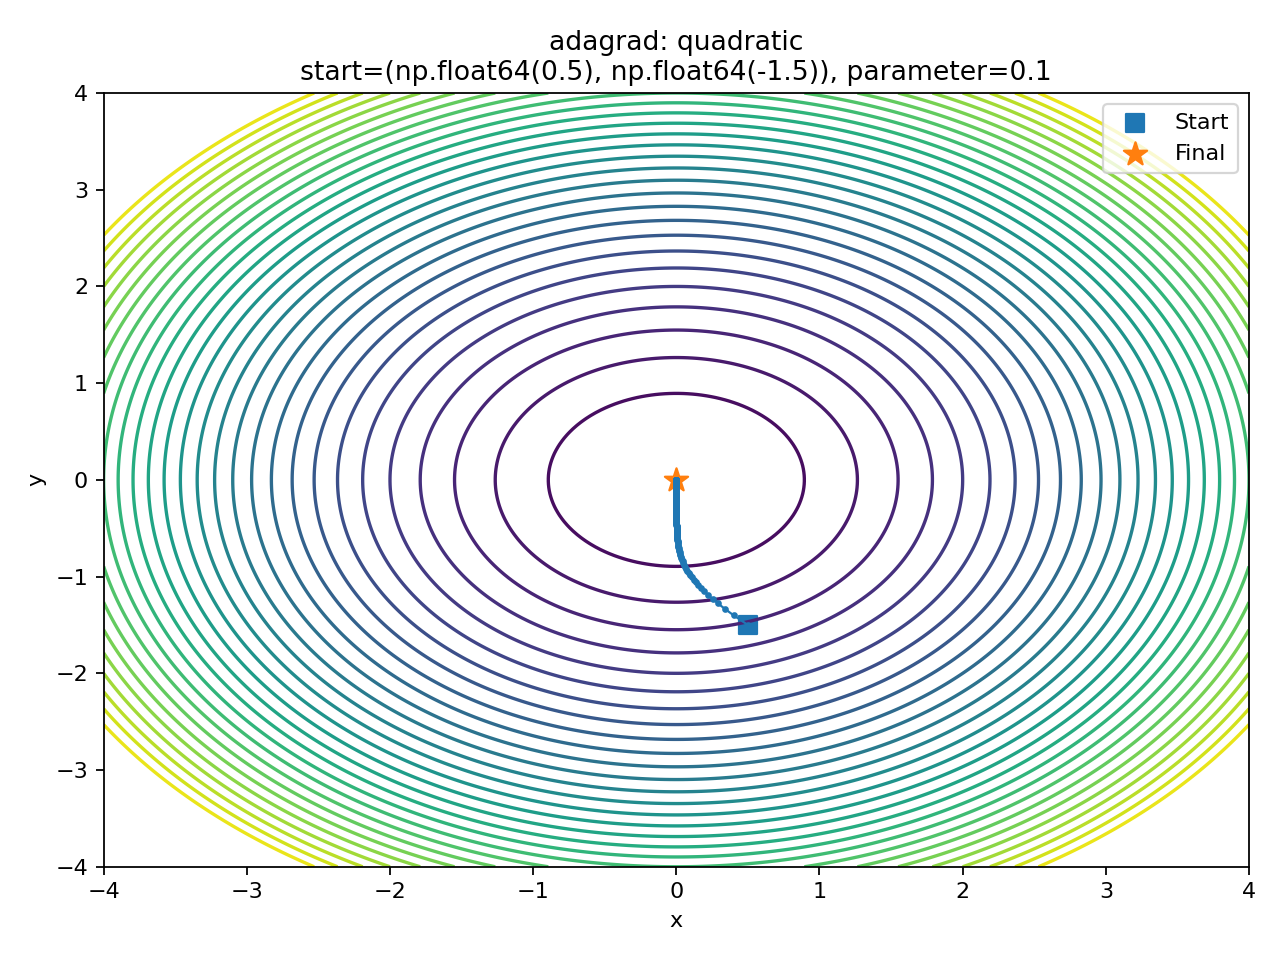
\includegraphics[width=0.40\textwidth]{output/adagrad/quadratic_start_0.5_neg1.5_lr_0.1.png}
    \caption{Adagrad on the Quadratic function}
    \label{fig:adagrad_quadratic}
\end{figure}

\subsubsection{Rosenbrock}
\begin{figure}[H]
    \centering
    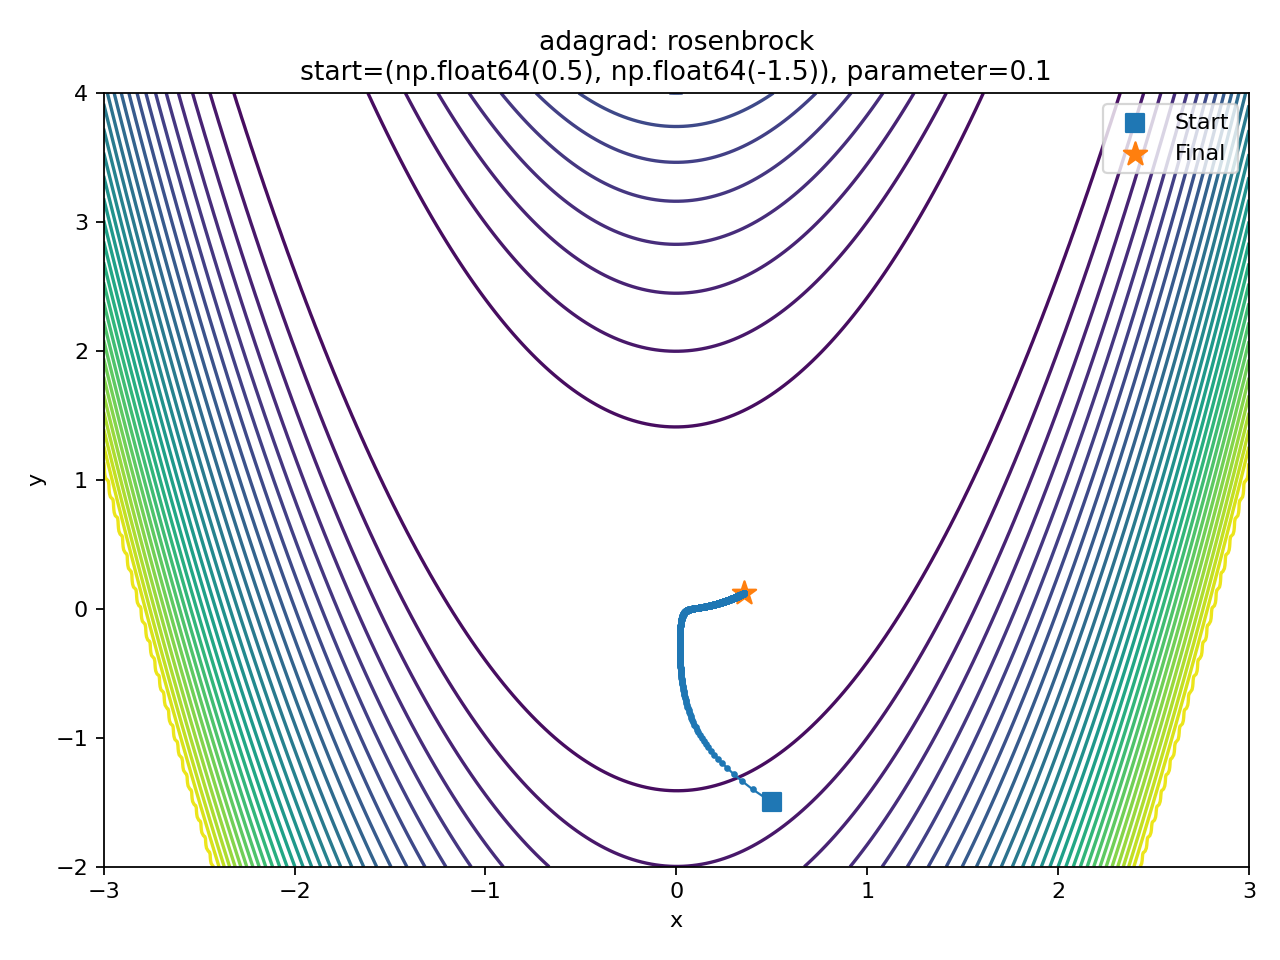
\includegraphics[width=0.40\textwidth]{output/adagrad/rosenbrock_start_0.5_neg1.5_lr_0.1.png}
    \caption{Adagrad on the Rosenbrock function}
    \label{fig:adagrad_rosenbrock}
\end{figure}

\begin{table}[H]
    \centering
    \caption{Adagrad results for $(x_0,y_0) = (-2,2)$.}
    \label{tab:adagrad_-2_2}
    \begin{tabular}{lcccc}
        \hline
        \textbf{Function} & \textbf{LR} & \textbf{Time (s)} &
        \textbf{Iterations} & \textbf{Final f(x,y)} \\
        \hline

        \multirow{3}{*}{Quadratic}
        & 0.001 & 0.01185 & 2000 & 7.317 \\
        & 0.01  & 0.01267 & 2000 & 2.864 \\
        & 0.1   & 0.007218 & 1098 & $1.252\times10^{-8}$ \\
        \hline

        \multirow{3}{*}{Rosenbrock}
        & 0.001 & 0.01255 & 2000 & 260.4 \\
        & 0.01  & 0.01238 & 2000 & 6.745 \\
        & 0.1   & 0.01226 & 2000 & 6.041 \\
        \hline

        \multirow{3}{*}{Cosine Bumps}
        & 0.001 & 0.01229 & 2000 & $-1.153$ \\
        & 0.01  & 0.01329 & 2000 & $-3.605$ \\
        & 0.1   & 0.0007854 & 117 & $-3.618$ \\
        \hline

    \end{tabular}
\end{table}

\begin{table}[H]
    \centering
    \caption{Adagrad results for $(x_0,y_0) = (0.5,-1.5)$.}
    \label{tab:adagrad_-05_-15}
    \begin{tabular}{lcccc}
        \hline
        \textbf{Function} & \textbf{LR} & \textbf{Time (s)} &
        \textbf{Iterations} & \textbf{Final f(x,y)} \\
        \hline

        \multirow{3}{*}{Quadratic}
        & 0.001 & 0.01215 & 2000 & 2.168 \\
        & 0.01  & 0.01176 & 2000 & 0.5288 \\
        & 0.1   & 0.003649 & 635 & $4.164\times10^{-9}$ \\
        \hline

        \multirow{3}{*}{Rosenbrock}
        & 0.001 & 0.01201 & 2000 & 252.1 \\
        & 0.01  & 0.01189 & 2000 & 56.78 \\
        & 0.1   & 0.01197 & 2000 & 0.4182 \\
        \hline

        \multirow{3}{*}{Cosine Bumps}
        & 0.001 & 0.01224 & 2000 & 11.01 \\
        & 0.01  & 0.01255 & 2000 & 1.910 \\
        & 0.1   & 0.003486 & 568 & $-3.618$ \\
        \hline

    \end{tabular}
\end{table}

\begin{table}[H]
    \centering
    \caption{Adagrad results for $(x_0,y_0) = (3, 3)$.}
    \label{tab:adagrad_3_3}
    \begin{tabular}{lcccc}
        \hline
        \textbf{Function} & \textbf{LR} & \textbf{Time (s)} &
        \textbf{Iterations} & \textbf{Final f(x,y)} \\
        \hline

        \multirow{3}{*}{Quadratic}
        & 0.001 & 0.01161 & 2000 & 16.96 \\
        & 0.01  & 0.01251 & 2000 & 9.407 \\
        & 0.1   & 0.01194 & 2000 & $5.987\times10^{-7}$ \\
        \hline

        \multirow{3}{*}{Rosenbrock}
        & 0.001 & 0.01216 & 2000 & 2925.2 \\
        & 0.01  & 0.01200 & 2000 & 307.7 \\
        & 0.1   & 0.01240 & 2000 & 1033.7 \\
        \hline

        \multirow{3}{*}{Cosine Bumps}
        & 0.001 & 0.01247 & 2000 & $-2.489$ \\
        & 0.01  & 0.01263 & 2000 & $-3.618$ \\
        & 0.1   & 0.0004805 & 74 & $-3.618$ \\
        \hline

    \end{tabular}
\end{table}


\subsection{ADAM}

\subsubsection{Cosine Bumps}
\begin{figure}[H]
    \centering
    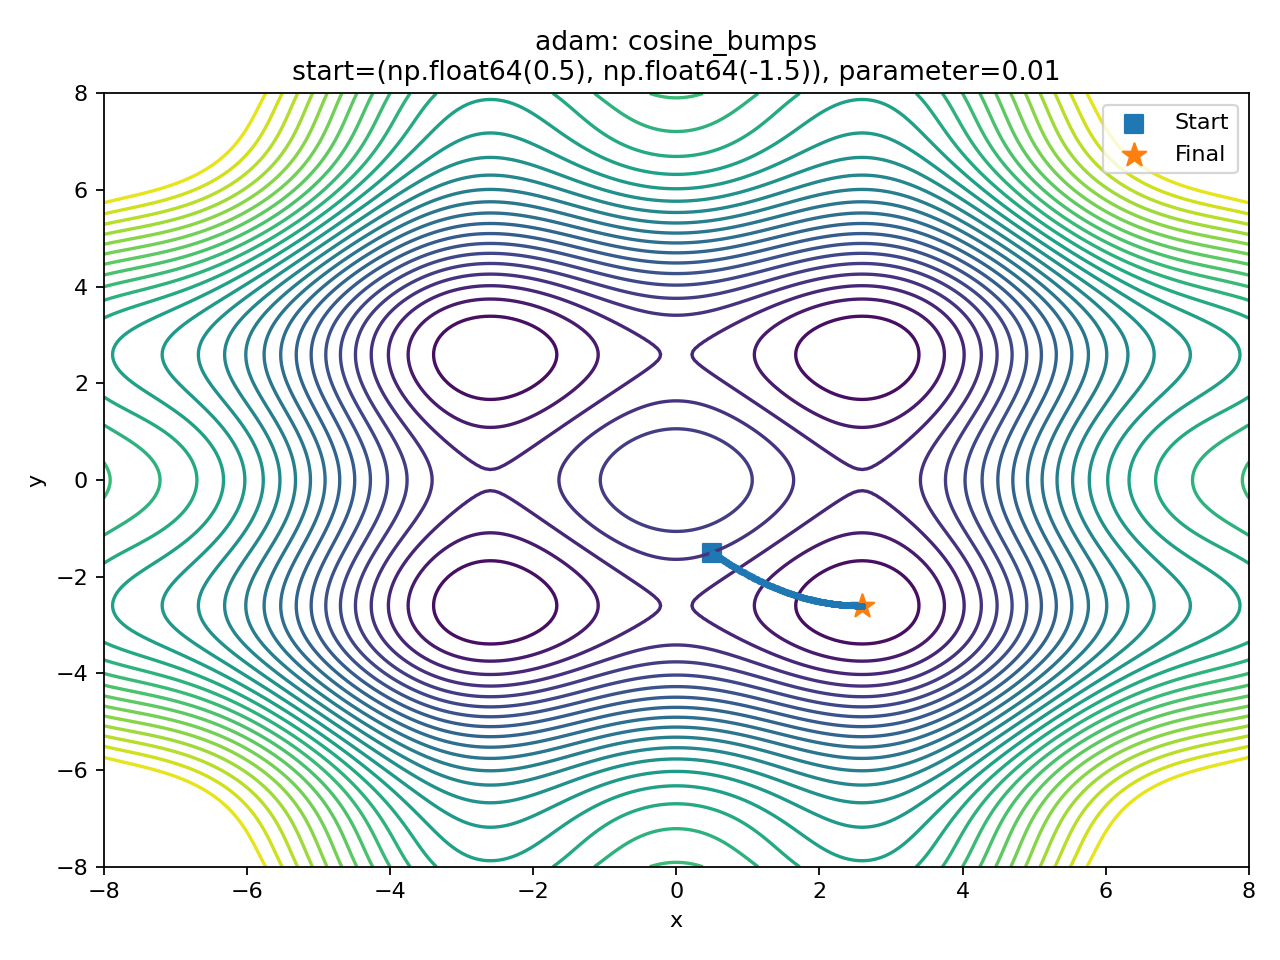
\includegraphics[width=0.40\textwidth]{output/adam/cosine_bumps_start_0.5_neg1.5_lr_0.01.png}
    \caption{ADAM on the Cosine Bumps function}
    \label{fig:adam_cosine}
\end{figure}

\subsubsection{Quadratic}
\begin{figure}[H]
    \centering
    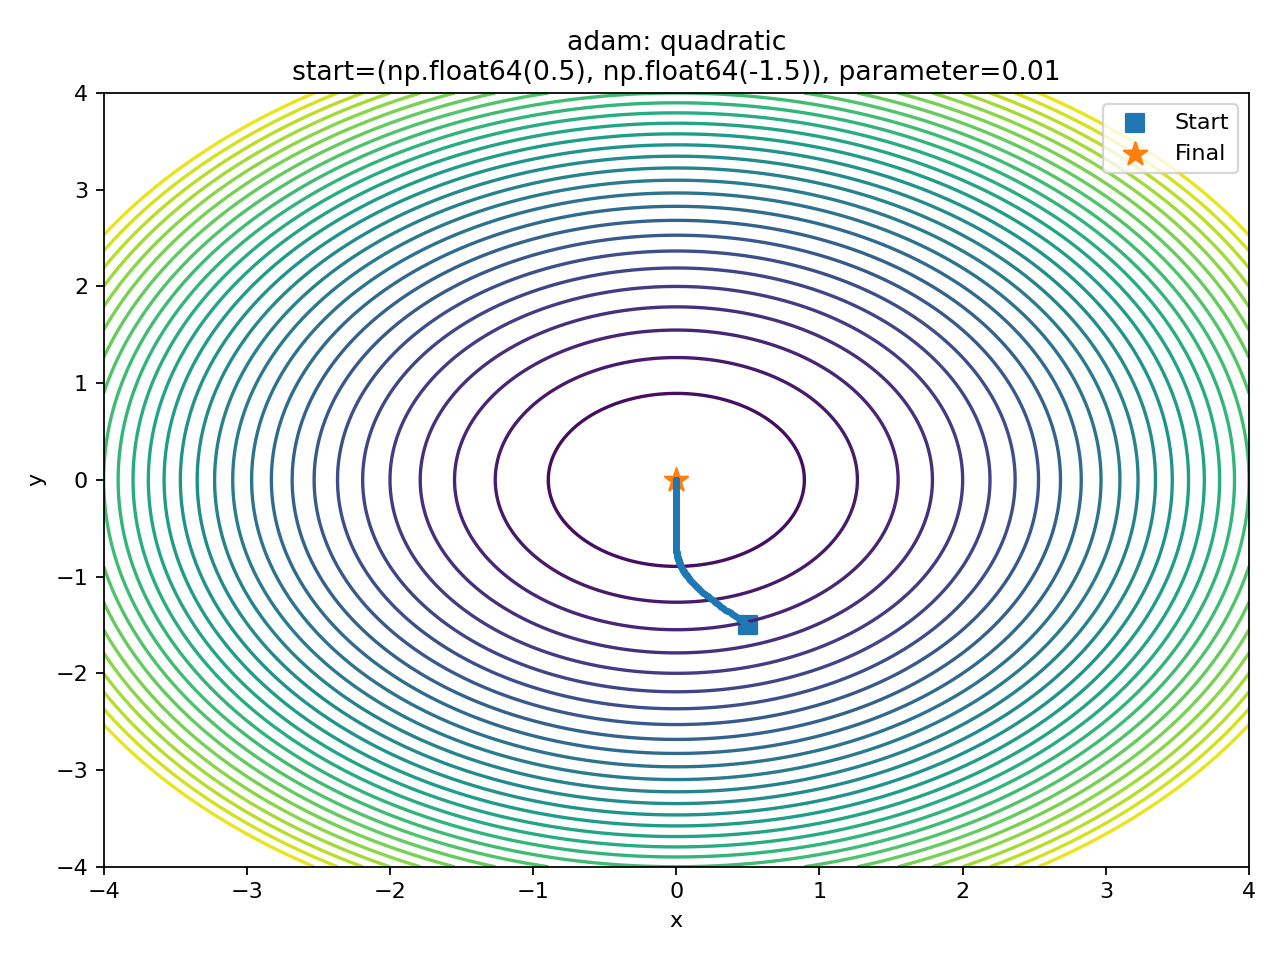
\includegraphics[width=0.40\textwidth]{output/adam/quadratic_start_0.5_neg1.5_lr_0.01.png}
    \caption{ADAM on the Quadratic function}
    \label{fig:adam_quadratic}
\end{figure}

\subsubsection{Rosenbrock}
\begin{figure}[H]
    \centering
    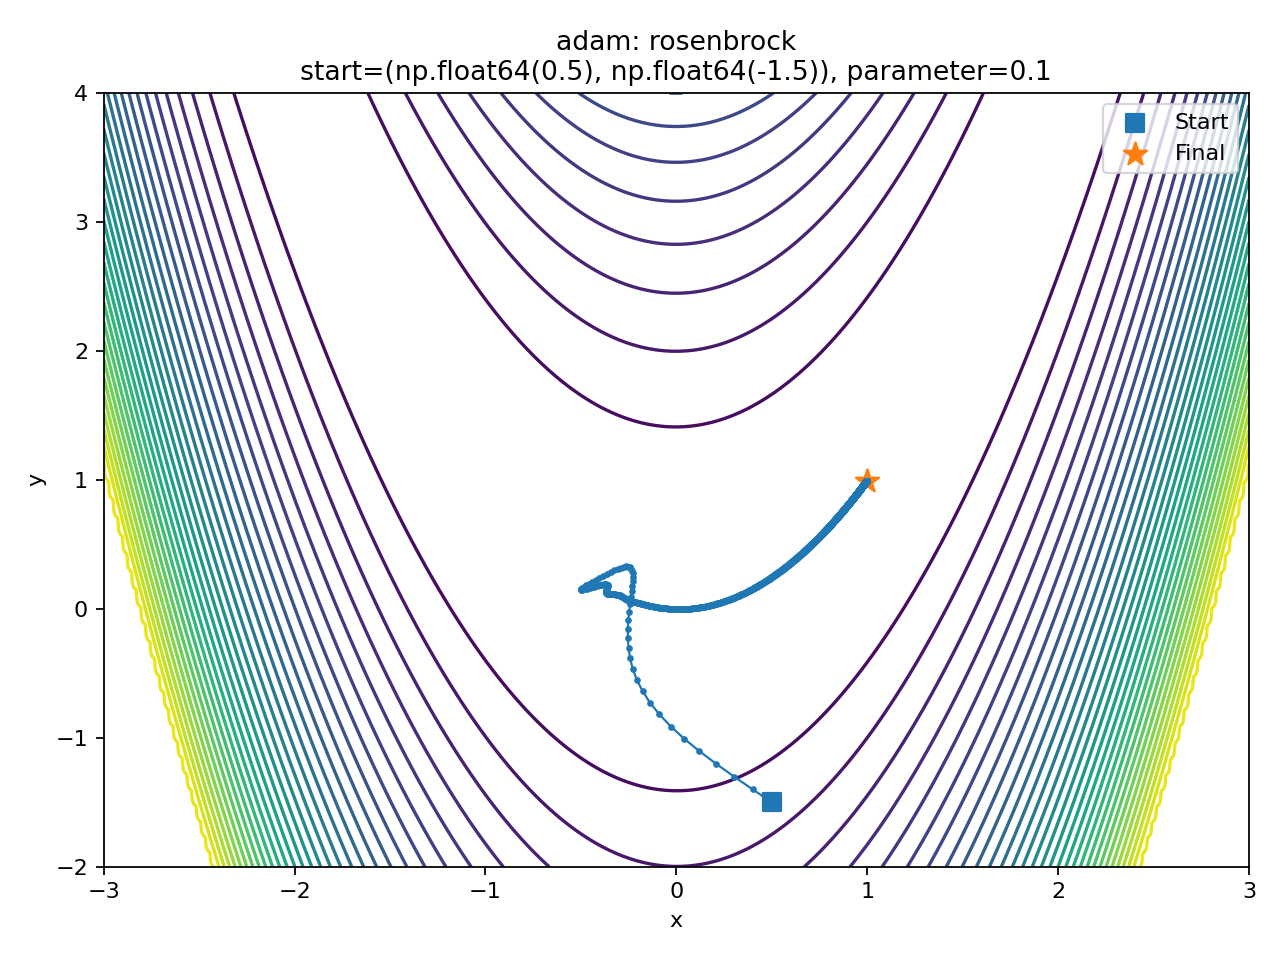
\includegraphics[width=0.40\textwidth]{output/adam/rosenbrock_start_0.5_neg1.5_lr_0.1.png}
    \caption{ADAM on the Rosenbrock function}
    \label{fig:adam_rosenbrock}
\end{figure}

\begin{table}[H]
    \centering
    \caption{Adam results for $(x_0,y_0) = (-2,2)$.}
    \label{tab:adam_neg2_2}
    \begin{tabular}{lcccc}
        \hline
        \textbf{Function} & \textbf{LR} & \textbf{Time (s)} &
        \textbf{Iterations} & \textbf{Final f(x,y)} \\
        \hline

        \multirow{3}{*}{Quadratic}
        & 0.001 & 0.01757 & 2000 & 0.4831 \\
        & 0.01  & 0.008406 & 796 & $1.545\times10^{-9}$ \\
        & 0.1   & 0.001583 & 181 & $5.123\times10^{-8}$ \\
        \hline

        \multirow{3}{*}{Rosenbrock}
        & 0.001 & 0.01945 & 2000 & 6.571 \\
        & 0.01  & 0.01893 & 2000 & 5.547 \\
        & 0.1   & 0.01836 & 2000 & 0.001933 \\
        \hline

        \multirow{3}{*}{Cosine Bumps}
        & 0.001 & 0.01738 & 1860 & $-3.618$ \\
        & 0.01  & 0.001654 & 180 & $-3.618$ \\
        & 0.1   & 0.001844 & 193 & $-3.618$ \\
        \hline

    \end{tabular}
\end{table}

\begin{table}[H]
    \centering
    \caption{Adam results for $(x_0,y_0) = (0.5,-1.5)$.}
    \label{tab:adam_05_neg15}
    \begin{tabular}{lcccc}
        \hline
        \textbf{Function} & \textbf{LR} & \textbf{Time (s)} &
        \textbf{Iterations} & \textbf{Final f(x,y)} \\
        \hline

        \multirow{3}{*}{Quadratic}
        & 0.001 & 0.01749 & 2000 & 0.03365 \\
        & 0.01  & 0.005208 & 569 & $7.937\times10^{-10}$ \\
        & 0.1   & 0.002129 & 230 & $7.964\times10^{-11}$ \\
        \hline

        \multirow{3}{*}{Rosenbrock}
        & 0.001 & 0.01837 & 2000 & 5.207 \\
        & 0.01  & 0.01894 & 2000 & 0.2454 \\
        & 0.1   & 0.01872 & 2000 & $6.877\times10^{-6}$ \\
        \hline

        \multirow{3}{*}{Cosine Bumps}
        & 0.001 & 0.01952 & 2000 & $-3.387$ \\
        & 0.01  & 0.004131 & 436 & $-3.618$ \\
        & 0.1   & 0.002267 & 242 & $-3.618$ \\
        \hline

    \end{tabular}
\end{table}

\begin{table}[H]
    \centering
    \caption{Adam results for $(x_0,y_0) = (3,3)$.}
    \label{tab:adam_3_3}
    \begin{tabular}{lcccc}
        \hline
        \textbf{Function} & \textbf{LR} & \textbf{Time (s)} &
        \textbf{Iterations} & \textbf{Final f(x,y)} \\
        \hline

        \multirow{3}{*}{Quadratic}
        & 0.001 & 0.01773 & 2000 & 3.411 \\
        & 0.01  & 0.01042 & 1202 & $3.622\times10^{-9}$ \\
        & 0.1   & 0.001952 & 215 & $4.328\times10^{-9}$ \\
        \hline

        \multirow{3}{*}{Rosenbrock}
        & 0.001 & 0.01836 & 2000 & 6.795 \\
        & 0.01  & 0.01797 & 2000 & 1.022 \\
        & 0.1   & 0.01848 & 2000 & 0.4296 \\
        \hline

        \multirow{3}{*}{Cosine Bumps}
        & 0.001 & 0.01411 & 1434 & $-3.618$ \\
        & 0.01  & 0.001653 & 172 & $-3.618$ \\
        & 0.1   & 0.001794 & 193 & $-3.618$ \\
        \hline

    \end{tabular}
\end{table}

\subsection{Gradient Descent}

\subsubsection{Cosine Bumps}
\begin{figure}[H]
    \centering
    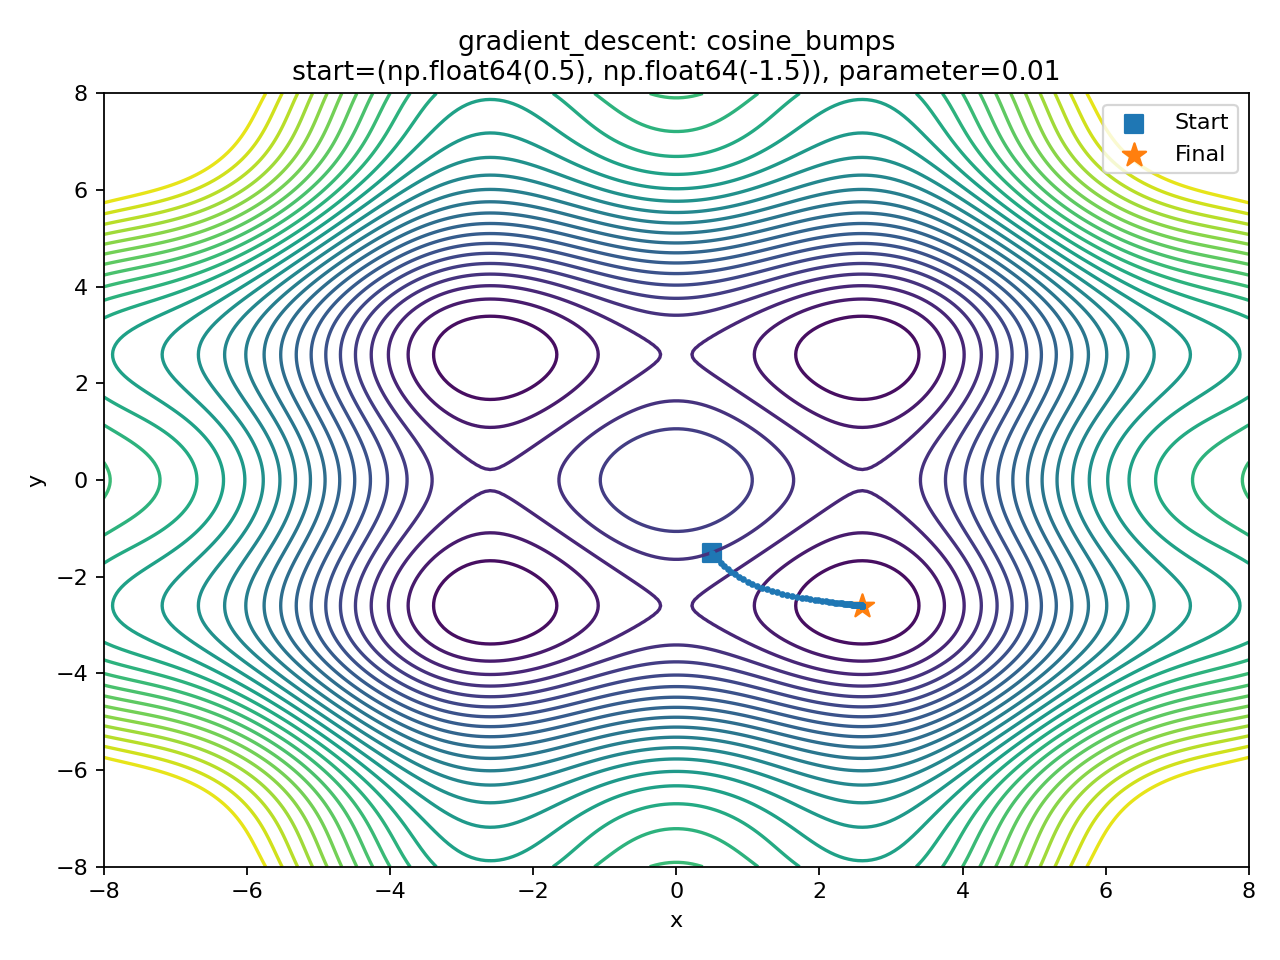
\includegraphics[width=0.40\textwidth]{output/gradient_descent/cosine_bumps_start_0.5_neg1.5_lr_0.01.png}
    \caption{Gradient Descent on the Cosine Bumps function}
    \label{fig:gd_cosine}
\end{figure}

\subsubsection{Quadratic}
\begin{figure}[H]
    \centering
    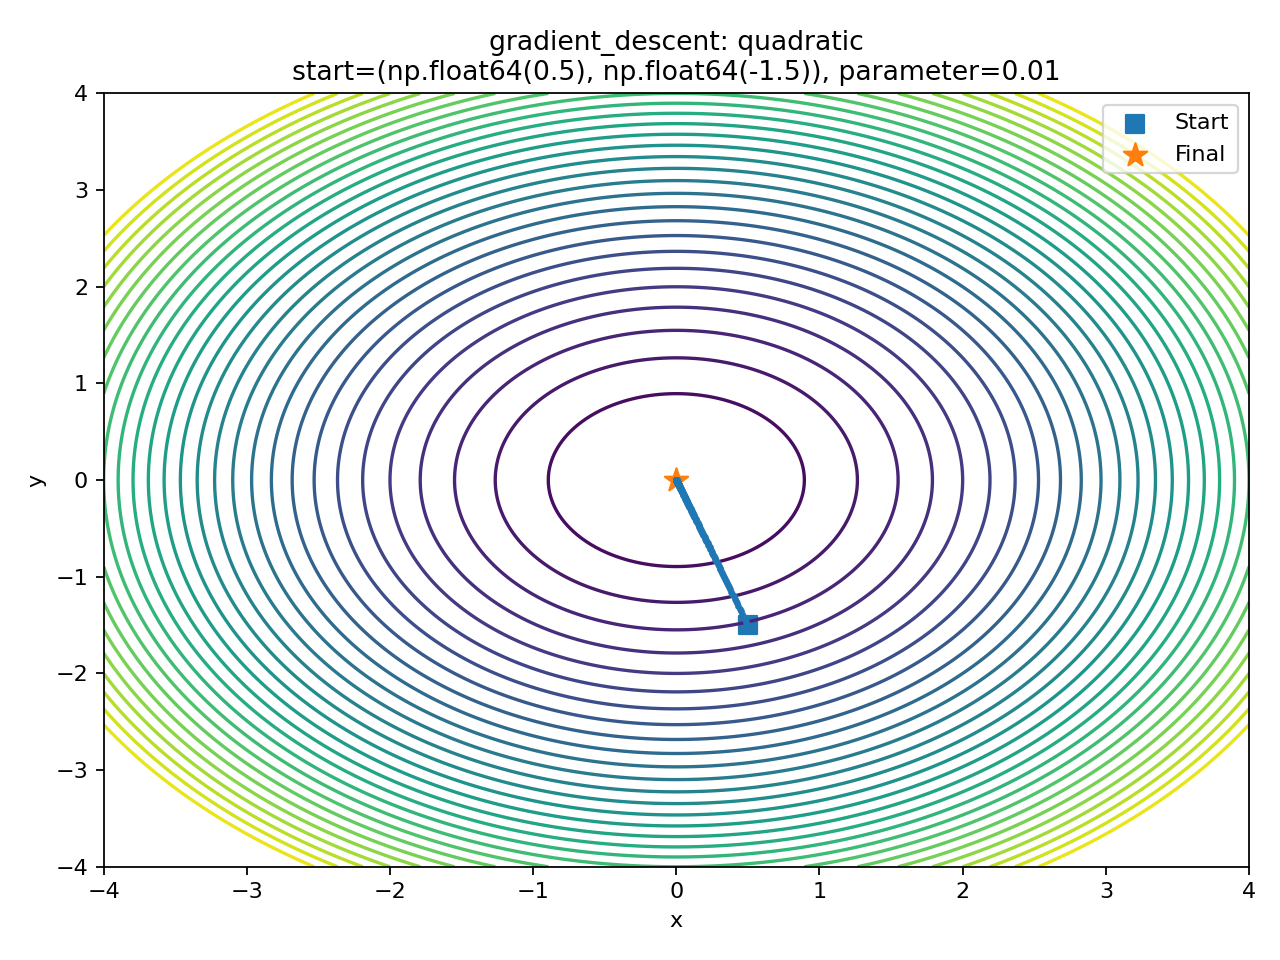
\includegraphics[width=0.40\textwidth]{output/gradient_descent/quadratic_start_0.5_neg1.5_lr_0.01.png}
    \caption{Gradient Descent on the Quadratic function}
    \label{fig:gd_quadratic}
\end{figure}

\subsubsection{Rosenbrock}
\begin{figure}[H]
    \centering
    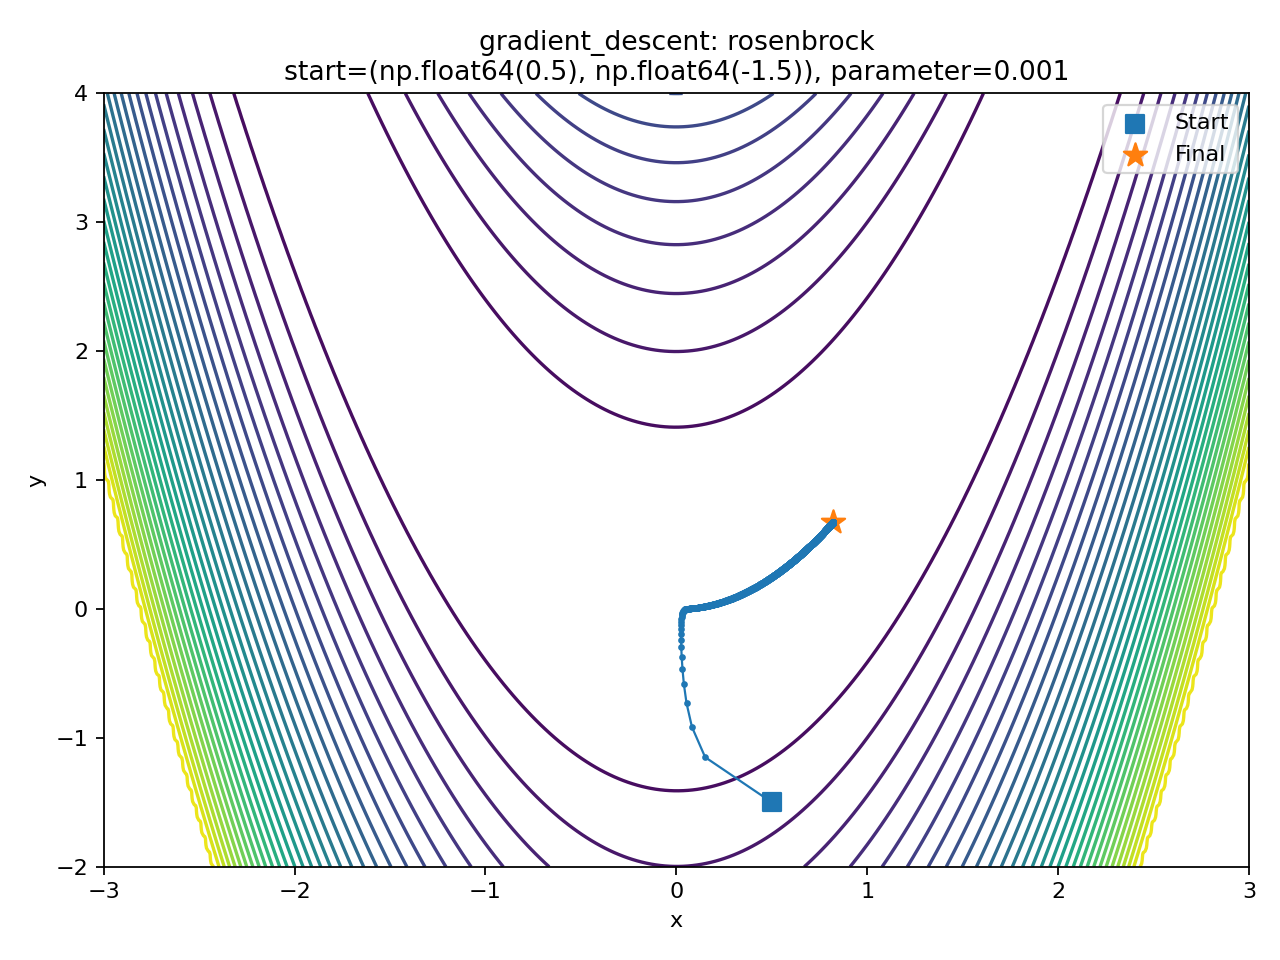
\includegraphics[width=0.40\textwidth]{output/gradient_descent/rosenbrock_start_0.5_neg1.5_lr_0.001.png}
    \caption{Gradient Descent on the Rosenbrock function}
    \label{fig:gd_rosenbrock}
\end{figure}

\begin{table}[H]
    \centering
    \caption{Gradient Descent results for $(x_0,y_0) = (-2,2)$.}
    \label{tab:gd_neg2_2}
    \begin{tabular}{lcccc}
        \hline
        \textbf{Function} & \textbf{LR} & \textbf{Time (s)} &
        \textbf{Iterations} & \textbf{Final f(x,y)} \\
        \hline

        \multirow{3}{*}{Quadratic}
        & 0.001 & 0.008853 & 2000 & 0.002662 \\
        & 0.01  & 0.002769 & 543 & $2.369\times10^{-9}$ \\
        & 0.1   & 0.0002992 & 61 & $1.202\times10^{-11}$ \\
        \hline

        \multirow{3}{*}{Rosenbrock}
        & 0.001 & 0.009413 & 2000 & 0.1283 \\
        & 0.01  & 0.0003998 & 6 & NaN \\
        & 0.1   & 0.009050 & 6 & NaN \\
        \hline

        \multirow{3}{*}{Cosine Bumps}
        & 0.001 & 0.004102 & 877 & $-3.618$ \\
        & 0.01  & 0.0005262 & 106 & $-3.618$ \\
        & 0.1   & 0.00007510 & 6 & $-3.618$ \\
        \hline

    \end{tabular}
\end{table}

\begin{table}[H]
    \centering
    \caption{Gradient Descent results for $(x_0,y_0) = (0.5,-1.5)$.}
    \label{tab:gd_05_neg15}
    \begin{tabular}{lcccc}
        \hline
        \textbf{Function} & \textbf{LR} & \textbf{Time (s)} &
        \textbf{Iterations} & \textbf{Final f(x,y)} \\
        \hline

        \multirow{3}{*}{Quadratic}
        & 0.001 & 0.008413 & 2000 & 0.0008320 \\
        & 0.01  & 0.002254 & 514 & $2.390\times10^{-9}$ \\
        & 0.1   & 0.0002855 & 58 & $1.433\times10^{-11}$ \\
        \hline

        \multirow{3}{*}{Rosenbrock}
        & 0.001 & 0.009246 & 2000 & 0.03175 \\
        & 0.01  & 0.00008010 & 7 & NaN \\
        & 0.1   & 0.00005880 & 6 & NaN \\
        \hline

        \multirow{3}{*}{Cosine Bumps}
        & 0.001 & 0.005419 & 1096 & $-3.618$ \\
        & 0.01  & 0.0006307 & 128 & $-3.618$ \\
        & 0.1   & 0.00008390 & 9 & $-3.618$ \\
        \hline

    \end{tabular}
\end{table}

\begin{table}[H]
    \centering
    \caption{Gradient Descent results for $(x_0,y_0) = (3,3)$.}
    \label{tab:gd_3_3}
    \begin{tabular}{lcccc}
        \hline
        \textbf{Function} & \textbf{LR} & \textbf{Time (s)} &
        \textbf{Iterations} & \textbf{Final f(x,y)} \\
        \hline

        \multirow{3}{*}{Quadratic}
        & 0.001 & 0.008602 & 2000 & 0.005990 \\
        & 0.01  & 0.002520 & 563 & $2.376\times10^{-9}$ \\
        & 0.1   & 0.0003094 & 63 & $1.108\times10^{-11}$ \\
        \hline

        \multirow{3}{*}{Rosenbrock}
        & 0.001 & 0.00005010 & 8 & NaN \\
        & 0.01  & 0.00003760 & 6 & NaN \\
        & 0.1   & 0.00005870 & 6 & NaN \\
        \hline

        \multirow{3}{*}{Cosine Bumps}
        & 0.001 & 0.004042 & 814 & $-3.618$ \\
        & 0.01  & 0.0005418 & 99 & $-3.618$ \\
        & 0.1   & 0.00007260 & 6 & $-3.618$ \\
        \hline

    \end{tabular}
\end{table}

\subsection{Newton}

\subsubsection{Cosine Bumps}
\begin{figure}[H]
    \centering
    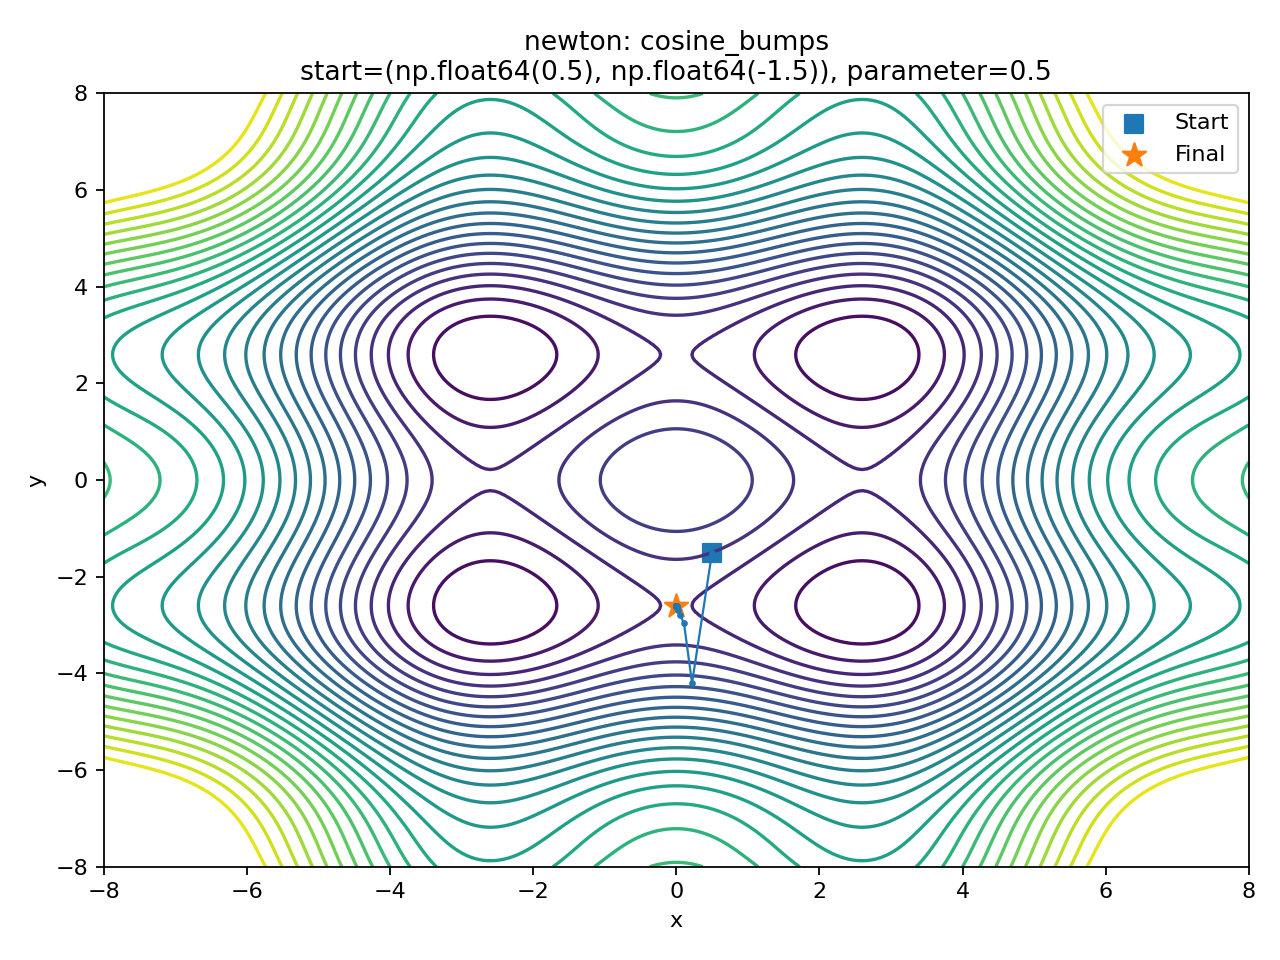
\includegraphics[width=0.40\textwidth]{output/newton/cosine_bumps_start_0.5_neg1.5_lr_0.5.png}
    \caption{Newton's Method on the Cosine Bumps function}
    \label{fig:newton_cosine}
\end{figure}

\subsubsection{Quadratic}
\begin{figure}[H]
    \centering
    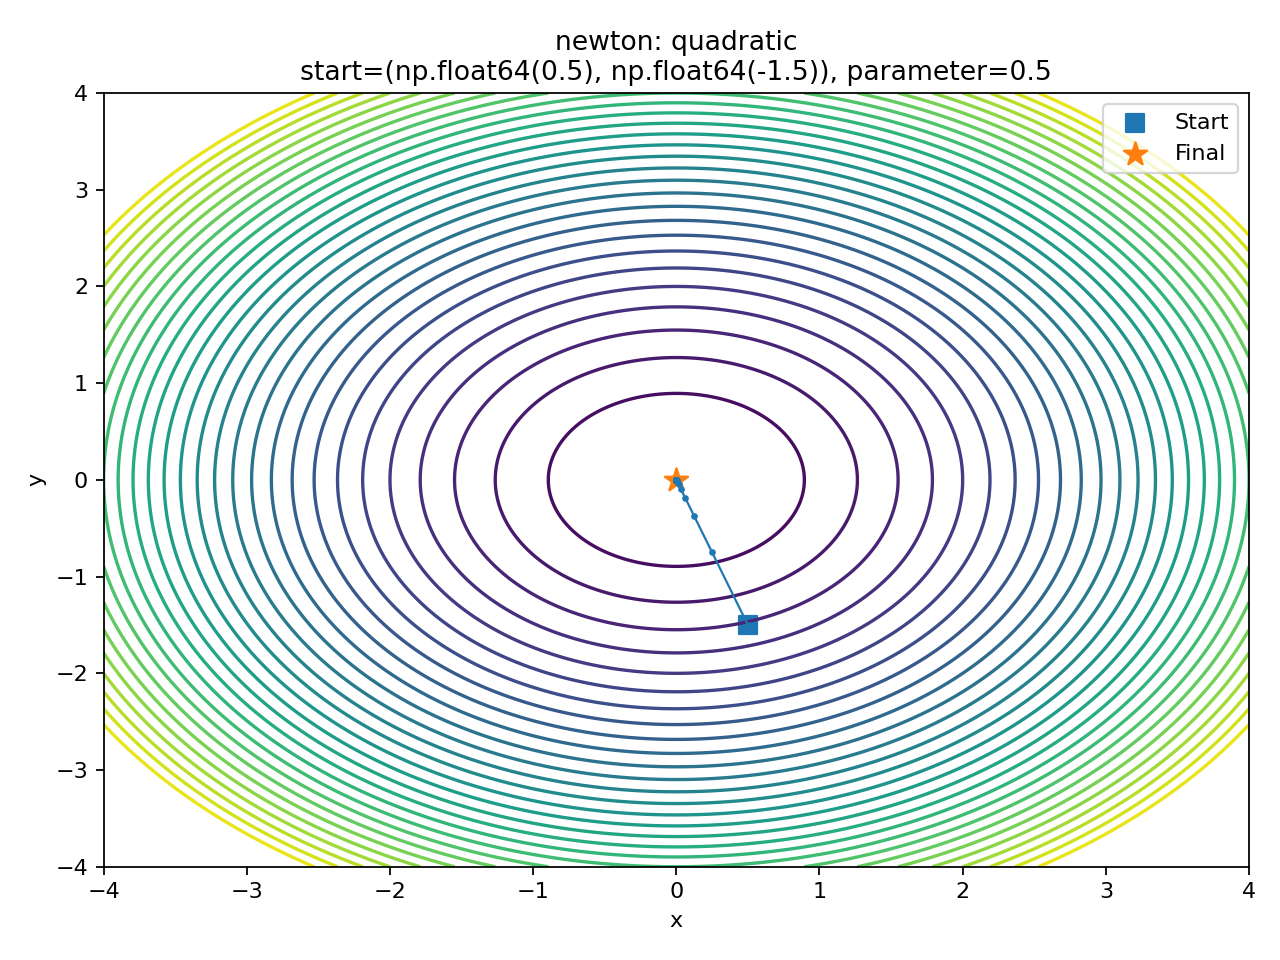
\includegraphics[width=0.40\textwidth]{output/newton/quadratic_start_0.5_neg1.5_lr_0.5.png}
    \caption{Newton's Method on the Quadratic function}
    \label{fig:newton_quadratic}
\end{figure}

\subsubsection{Rosenbrock}
\begin{figure}[H]
    \centering
    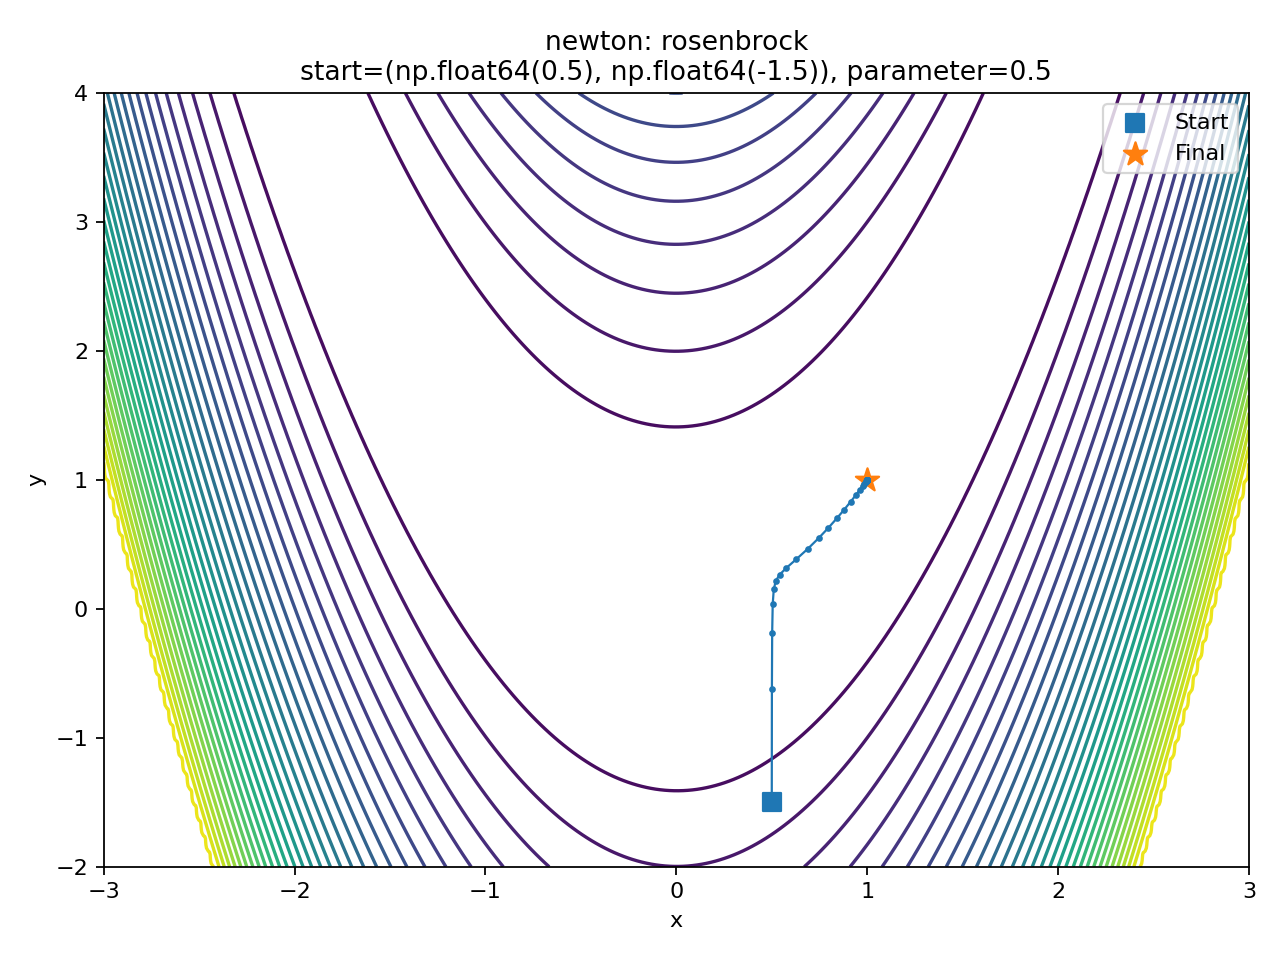
\includegraphics[width=0.40\textwidth]{output/newton/rosenbrock_start_0.5_neg1.5_lr_0.5.png}
    \caption{Newton's Method on the Rosenbrock function}
    \label{fig:newton_rosenbrock}
\end{figure}

\begin{table}[H]
    \centering
    \caption{Newton results for $(x_0,y_0) = (-2,2)$.}
    \label{tab:newton_neg2_2}
    \begin{tabular}{lcccc}
        \hline
        \textbf{Function} & \textbf{LR} & \textbf{Time (s)} &
        \textbf{Iterations} & \textbf{Final f(x,y)} \\
        \hline

        \multirow{3}{*}{Quadratic}
        & 0.25 & 0.0005381 & 48 & $8.109\times10^{-12}$ \\
        & 0.5  & 0.0003780 & 22 & $4.547\times10^{-13}$ \\
        & 1.0  & 0.00008460 & 2 & 0 \\
        \hline

        \multirow{3}{*}{Rosenbrock}
        & 0.25 & 0.0009911 & 102 & $1.791\times10^{-12}$ \\
        & 0.5  & 0.0005581 & 54 & $1.540\times10^{-13}$ \\
        & 1.0  & 0.0001111 & 6 & 0 \\
        \hline

        \multirow{3}{*}{Cosine Bumps}
        & 0.25 & 0.0004562 & 43 & $-3.618$ \\
        & 0.5  & 0.0002393 & 19 & $-3.618$ \\
        & 1.0  & 0.0001156 & 5 & $-3.618$ \\
        \hline

    \end{tabular}
\end{table}

\begin{table}[H]
    \centering
    \caption{Newton results for $(x_0,y_0) = (0.5,-1.5)$.}
    \label{tab:newton_05_neg15}
    \begin{tabular}{lcccc}
        \hline
        \textbf{Function} & \textbf{LR} & \textbf{Time (s)} &
        \textbf{Iterations} & \textbf{Final f(x,y)} \\
        \hline

        \multirow{3}{*}{Quadratic}
        & 0.25 & 0.0005968 & 46 & $8.009\times10^{-12}$ \\
        & 0.5  & 0.0002286 & 21 & $5.684\times10^{-13}$ \\
        & 1.0  & 0.00007750 & 2 & 0 \\
        \hline

        \multirow{3}{*}{Rosenbrock}
        & 0.25 & 0.0007514 & 70 & $1.749\times10^{-12}$ \\
        & 0.5  & 0.0003686 & 34 & $9.316\times10^{-14}$ \\
        & 1.0  & 0.0001111 & 5 & 0 \\
        \hline

        \multirow{3}{*}{Cosine Bumps}
        & 0.25 & 0.0004815 & 43 & 8.191 \\
        & 0.5  & 0.0002492 & 21 & 8.191 \\
        & 1.0  & 0.001856 & 198 & 8.191 \\
        \hline

    \end{tabular}
\end{table}

\begin{table}[H]
    \centering
    \caption{Newton results for $(x_0,y_0) = (3,3)$.}
    \label{tab:newton_3_3}
    \begin{tabular}{lcccc}
        \hline
        \textbf{Function} & \textbf{LR} & \textbf{Time (s)} &
        \textbf{Iterations} & \textbf{Final f(x,y)} \\
        \hline

        \multirow{3}{*}{Quadratic}
        & 0.25 & 0.0004530 & 50 & $5.773\times10^{-12}$ \\
        & 0.5  & 0.0002949 & 23 & $2.558\times10^{-13}$ \\
        & 1.0  & 0.00007740 & 2 & 0 \\
        \hline

        \multirow{3}{*}{Rosenbrock}
        & 0.25 & 0.0009182 & 95 & $1.789\times10^{-12}$ \\
        & 0.5  & 0.0004774 & 49 & $1.037\times10^{-13}$ \\
        & 1.0  & 0.0001174 & 6 & 0 \\
        \hline

        \multirow{3}{*}{Cosine Bumps}
        & 0.25 & 0.0005216 & 43 & $-3.618$ \\
        & 0.5  & 0.0002938 & 20 & $-3.618$ \\
        & 1.0  & 0.00009760 & 4 & $-3.618$ \\
        \hline

    \end{tabular}
\end{table}

\section{Experimental Analysis}
Looking at the plots from the previous Results, we can see that the Gradient Descent algorithm
produces the simplest pathes through the contours of each function, with little to no oscillation.
In fact, despite being the simplest algorithm, it tends to outperform the others when looking at
the number of iterations to convergence and final function value.

Looking at the Rosenbrock function in Tables \ref{tab:adam_neg2_2}, \ref{tab:adam_05_neg15}, and \ref{tab:adam_3_3},
we see that Adam's performance is extremely variable, which is to be expected with the Rosenbrock function's
peculiar nature.

Furthermore, we can see that, for the Adagrad and Newton algorithms on the Cosine Bumps function,
the initial point is very important and can lead to vastly different end results.

Overall, it looks like the Newton's Method algorithm converges in the least amount of iterations,
whilst Adagrad takes the most amount of iterations. In terms of runtime,
Gradient Descent and Newton's methods are about an order of magnitude or two faster than Adam and Adagrad.

\section{Conclusion}
In conclusion, our findings are mostly in line with our expectations. Gradient Descent is the simplest algorithm,
and therefore the fastest. We notice that it tends to perform the best
across the other algorithms - perhaps since the functions tested aren't too nonconvex. However, Gradient Descent gave poor results on the Rosenbrock function, which could be attributed to
potential overflow in the gradient calculations. 

Newton's Method had the fastest raw convergence numbers, but saw greater variability in the
Cosine Bumps function based off the initial starting point. This is a potentially acceptable
tradeoff.

Adagrad's performance was mostly non-remarkable. With the right hyeprparameters, it found good solutions
for the Quadratic and Cosine Bumps functions, but it struggled with Rosenbrock. Perhaps its
advantages lie in its computational efficiency compared to algorithms like Adam, however computational
efficiency was of little concern in these experiments.

Adam could best be described as the Goldilocks of the algorithms we tested, achieving solid final results
consistently, albeit more slowly than Gradient Descent or Newton's Method. Its trajectories show us that
it is more robust to the initial starting point than Newton's Method, but that it still slightly struggles with
Rosenbrock.

In order to further detect the ideal use cases of each algorithm, we could believe it would be beneficial to
experiment with more wacky (nonconvex) functions to see how the complex algorithms perform,
such as the \href{https://www.sfu.ca/~ssurjano/schwef.html}{Schwefel function}. We hypothesize that the bells
and whistles of the more complex algorithms aren't as useful
for the functions tested here, and that Adagrad and Adam would prove more useful in larger neural network type applications.

\section*{Acknowledgment}

We would like to thank and acknowledge our professor Dr. Olfa Nasraoui for her guidance and support throughout this project.

\clearpage
\onecolumn

\appendix

\section{Our Code}
\begin{lstlisting}[language=Python, caption={Gradient Descent implementation}, label={lst:gradient_descent}]
def gradient_descent(func, grad, start, learning_rate):
    x = start.astype(float).copy()
    path = [x.copy()]

    start_time = time.perf_counter()
    converged = False

    for iteration in range(1, MAX_ITER + 1):
        new_x = x - learning_rate * grad(x)
        path.append(new_x.copy())

        if not np.all(np.isfinite(new_x)):
            x = new_x
            break

        if np.linalg.norm(new_x - x) < TOL:
            x = new_x
            converged = True
            break

        x = new_x

    runtime = time.perf_counter() - start_time
    return x, path, iteration, converged, runtime
\end{lstlisting}

\begin{lstlisting}[language=Python, caption={Newton's Method implementation}, label={lst:newtons_method}]
def newtons_method(func, grad, hess, start, damping):
    x = start.astype(float).copy()
    path = [x.copy()]

    start_time = time.perf_counter()
    converged = False

    for iteration in range(1, MAX_ITER + 1):
        g = grad(x)
        H = hess(x)

        try:
            step = np.linalg.solve(H, g)
        except np.linalg.LinAlgError:
            # Pseudoinverse allows the experiment to continue if Hessian is singular.
            step = np.linalg.pinv(H) @ g

        new_x = x - damping * step
        path.append(new_x.copy())

        if not np.all(np.isfinite(new_x)):
            x = new_x
            break

        if np.linalg.norm(new_x - x) < TOL:
            x = new_x
            converged = True
            break

        x = new_x

    runtime = time.perf_counter() - start_time
    return x, path, iteration, converged, runtime
\end{lstlisting}

\begin{lstlisting}[language=Python, caption={AdaGrad implementation}, label={lst:adagrad}]
def adagrad(func, grad, start, learning_rate, epsilon=1e-8):
    x = start.astype(float).copy()
    accumulated_sq_grad = np.zeros_like(x)
    path = [x.copy()]

    start_time = time.perf_counter()
    converged = False

    for iteration in range(1, MAX_ITER + 1):
        g = grad(x)
        accumulated_sq_grad += g * g
        adjusted_step = learning_rate * g / (np.sqrt(accumulated_sq_grad) + epsilon)
        new_x = x - adjusted_step
        path.append(new_x.copy())

        if not np.all(np.isfinite(new_x)):
            x = new_x
            break

        if np.linalg.norm(new_x - x) < TOL:
            x = new_x
            converged = True
            break

        x = new_x

    runtime = time.perf_counter() - start_time
    return x, path, iteration, converged, runtime
\end{lstlisting}

\begin{lstlisting}[language=Python, caption={Adam implementation}, label={lst:adam}]
def adam(func, grad, start, learning_rate,
         beta1=0.9, beta2=0.999, epsilon=1e-8):
    x = start.astype(float).copy()
    m = np.zeros_like(x)
    v = np.zeros_like(x)
    path = [x.copy()]

    start_time = time.perf_counter()
    converged = False

    for iteration in range(1, MAX_ITER + 1):
        g = grad(x)

        m = beta1 * m + (1 - beta1) * g
        v = beta2 * v + (1 - beta2) * (g * g)

        m_hat = m / (1 - beta1 ** iteration)
        v_hat = v / (1 - beta2 ** iteration)

        new_x = x - learning_rate * m_hat / (np.sqrt(v_hat) + epsilon)
        path.append(new_x.copy())

        if not np.all(np.isfinite(new_x)):
            x = new_x
            break

        if np.linalg.norm(new_x - x) < TOL:
            x = new_x
            converged = True
            break

        x = new_x

    runtime = time.perf_counter() - start_time
    return x, path, iteration, converged, runtime
\end{lstlisting}

\end{document}
